\chapter{Smart Grid  Security}

The transition from the \acrlong{pg} to the \acrlong{sg}, opens the vintage closed and  proprietary energy distribution infrastructure to the Internet, in order to make the grid available for monitoring and control purposes. This transition exposes the grid to new threats, most notably the threats from external threat actors now able to attack the infrastructure from remote locations. 

\section{Classic Power Grid Security}
Traditionally, the operational sites of any \acrfull{ics}, like the \acrlong{pg}, has been closed systems, not connected to public networks like the Internet. 
The principle of "Security by Obscurity" has, as explained by  \citeauthor{humayed2017cyber}  in \cite{humayed2017cyber}, has been a dominant design principle for the traditional, offline, \acrlong{ics}.
As further explained  in \cite{humayed2017cyber}, most attacks on Industrial Control Systems, has been internal prior to 2001. Consequently, over the years following 2001, most of the attacks on \acrshort{pg} has been of external origin.
As explained by \citeauthor{knapp2015industrial} in \cite{knapp2015industrial}, \acrshort{ics}s has traditionally been airgapped systems, not designed for the continuous software and operating system updates so characteristic of any contemporary computer system. 

The increased vulnerabilities to external threats observable as a consequence of connecting the grid to the Internet, has resulted in numerous activities related to securing the grid, wile reaping the substantial benefits of keeping the grid online. 


\section{Industrial Control System (ICS) Security}

\section{Smart Grid  Security} 

\subsection{Smart Grid Security Requirements}
In order to protect the grid form new threat scenarios, a set of new security requirements needs to be defined in order to address the new situation. 
 
In \cite{Shapsough2015}, \citeauthor{Shapsough2015}  describes some information security concepts related to \acrlong{sg} security, defining the requirements in order to ensure the information security of the \acrshort{sg}. Thus, the \acrlong{sg} information security requirements might be summarised as follows:

\begin{itemize}
    \item \textbf{Availability} of the \acrlong{sg} is mandatory, as a violation of \acrlong{sg} availability implies a disruption of electricity. The immediate recovery from the lack of availability, is critical to the continued operation of a large number of services in a modern society.  
    \item \textbf{Integrity} violations in the \acrshort{sg} might affect power management, due to unauthorised modifications by illegitimate users. 
    \item \textbf{Confidentiality} violations will affect the privacy of users. Asides from the annoyance of privacy violations, power grid usage information might be indicative of empty buildings which could be a nice target for thieves. \item \textbf{Authentication} violations enables unauthorised access to private information, as well as \acrfull{sg} resources.
    \item \textbf{Authorisation} implements access control, preventing improper access to and management of \acrshort{sg} resources by unauthorised individuals.      \item \textbf{Non-Repudiation} violations enables individuals to deny being accessing or utilising \acrshort{sg} resources. Being able to track down actions of individual actors accessing \acrshort{sg} is vital due to the criticality of the \acrshort{sg}.
\end{itemize}



\subsection{Cyber Physical Systems security}

\begin{figure}[ht]
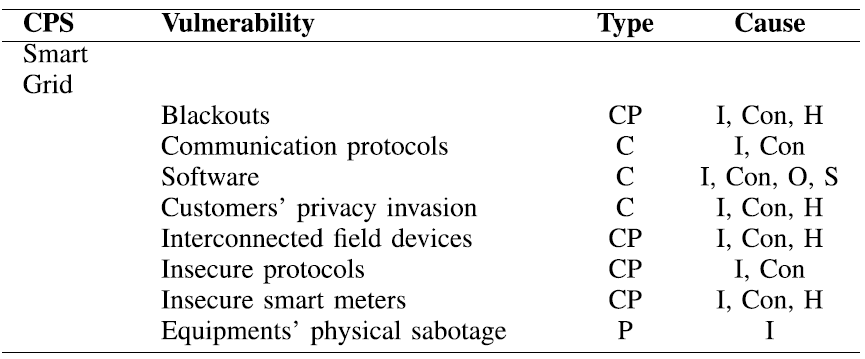
\includegraphics[width=\linewidth]{figures/CP-Vulnerabilities-SG.png}
\caption[\acrlong{cps} vulnerabilities for the \acrlong{sg}]{\acrlong{cps} vulnerabilities for the \acrlong{sg}, with causes. \cite[p. 1809]{humayed2017cyber}}
\label{fig:CP-Vulnerabilities-SG.png}
\end{figure}

Figure \ref{fig:CP-Vulnerabilities-SG.png} lists \acrlong{cps} vulnerabilities, Type classifications (C:CYBER, CP: CYBER-PHYSICAL, P: PHYSICAL, I: ISOLATION) and Causes (Con: CONNECTIVITY, O: OPENNESS, H: HETEROGENEITY,  S: MANY STAKEHOLDERS).




\subsection{WAMS Security} 

The \acrfull{sg} \acrfull{wams} is a \acrshort{sg} subsystem enabling \acrshort{sg} system operators to monitor the state of \acrshort{sg} energy flow, and general system state. 
A vital requirement for the view of the current state of the \acrshort{sg} energy distribution to be correct is, as described in previous chapters, the ability of the \acrshort{wams} Super \acrshort{pdc}  to utilise synchrophasors collected from the \acrshort{pdc}s to produce a view of the system state. In order for the view to be correct, however, the correctness of the timestamps i critical.  Therefore, in order to produce correct time stamps, the reliability of the Time Synchronisation source is of Critical importance.


% In \cite{el2018cyber}, \citeauthor{el2018cyber} ...
 


%\subsection{Threats to security}
%In order to ensure the continuous operation of the \acrlong{sg}, identifying security vulnerabilities, and countering threats identified is of vital importance.  






%\subsubsection{Time Synchronisation attacks}
\section{Cyber Attacks targeting Smart Grid}

The two-way communication lines of the\acrlong{sg} systems opens the possibilities of communication between the networks of energy distributors and the networks of consumers, serving purposes as automatic measurement of energy consumption, as well as dynamic adaption of energy production according to variations in demand for energy over the hours of the day.
The transition from networks managed by closed communication channels to networks communicating over IP-based networks, exposes\acrlong{sg} networks to Cyber attack vulnerabilities.



Malicious threat actors having privileged access to the infrastructure, is able to perform various kinds of internal attacks. Traditionally, anyone aiming to attack the \acrlong{pg} infrastructure, was obliged to get physical access to the premises, from which the infrastructure in question was controlled. Following the transition to the online \acrshort{sg}, the network connecting the grid to the outside might be utilised in order to execute any Cyber attack requiring internal privileged access from the outside.


\subsection{External Attacks}
External attacks is characterised by malicious actors attacking the infrastructure from the outside, without having the privileged access required in order to target internal system vulnerabilities.




\subsubsection{Denial of Service (DoS) Attack}

\subsubsection{GNSS Spoofing attacks}

\subsection{Internal Attacks}
The distinction between external and internal attacks, is the level of access required in order to perform the attack in question.

\subsubsection{Man in The Middle (MiTM) Attack}


 \section{Time Synchronisation attack Vulnerabilities}
%\subsubsection{Syncophasors}
%\subsubsection{Phasor Measurement Units}












 


 
\subsection{Attacks targeting the GNSS system}

In \cite{schmidt2016survey}, \citeauthor{schmidt2016survey} highlights jamming and spoofing as vulnerabilities affecting the service quality of GNSS systems:


\subsubsection{GNSS Jamming}
GNSS Jamming denotes the deliberate act of disturbing the signals from one or more GNSS satellites, lowering system reliability, utlimately rendering the GNSS devices\footnote{Devices utilising the GNSS system} useless. 
\subsubsection{GNSS Spoofing} 
GNSS Spoofing denotes the deliberate act of modifying, or replacing, the signal of one or more satellites, which could result in GNSS device position or timestamp calculation errors. Ultimately the GPS spoofing remains undetected for a sufficient time frame in order to achieve the desired effect on the target.



\subsection{Attacks targeting the PTP systems}


Several attacks targeting the \acrlong{ptp} are being described by \citeauthor{alghamdi2021precision} in \cite{alghamdi2021precision}:









Attack types:
\begin{itemize}
    \item \textbf{Simple internal attack}  
    \item \textbf{Advanced internal attack}
    \item \textbf{External attack} 
\end{itemize}

Attacker types:
\begin{itemize}
    \item \textbf{man in the middle attacker}  
    \item \textbf{packet injector attacker}
\end{itemize}


Safeguards: \textit{SEVERAL SAFEGUARDS TO BE DESCRIBED}




In \cite{alghamdi2021precision}, \citeauthor{alghamdi2021precision} specifies the following attack types:

\begin{itemize}

\item A \textbf{Packet Content Manipulation Attack} involves the modification of network packets affecting suitable timeprotocol fields, mainly related to the alteration of time synchronisation values. 
\item A \textbf{Packet Removal Attack} constitutes the removal of time protocol packages, thereby introducing time synchronisation errors.
\item A \textbf{Packet Delay Manipulation Attack} involves deliberately delaying the transmission of time protocol packets, thereby introducing time synchronisations error caused by the late arrival of some packets.
\item A \textbf{Time Source Degradation Attack} is the result of a time source degradation, deliberately altering the time of a master time source, thereby deliberately degrading the quality of a number of downstream clock associated with the master time source. 
\item A \textbf{Master Spoofing Attack} involves the deliberate replacement of the true master time source with a phony one.   
\item A \textbf{Slave Spoofing Attack} involves the deliberate replacement of the true slave time source with a phony one. 
\item a \textbf{Replay Attack} involves the delayed un-altered transmission of prerecorded packets, thereby intorducing time synchronisation errors.
\item a \textbf{BMCA Attack} involves the deliberate tampering of the master clock selection algorithm, introducing a new master clock, thereby taking control over time synchronisation.
\item A \textbf{Denial of Service Attack} involves the deliberate interruption of access to the service under attack in a number of ways, as described in the previous chapter.
\end{itemize}





